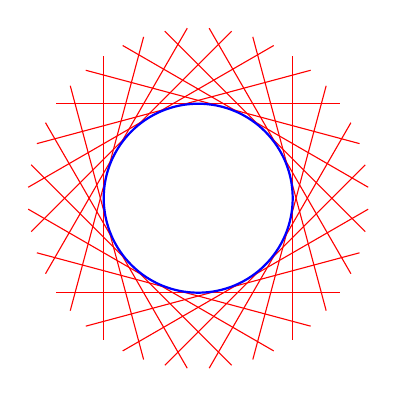
\begin{tikzpicture}[scale=1.20]
  % Lineas iniciales
  \draw[red] (-1,-1.5) -- (-1,1.5);
  \draw[red] (1,-1.5)  -- (1,1.5);
  \draw[red] (-1.5,1)  -- (1.5,1);
	\draw[red] (-1.5,-1) -- (1.5,-1);

	\begin{scope}[rotate around={15:(0,0)}]
		\draw[red] (-1,-1.5) -- (-1,1.5);
		\draw[red] (1,-1.5)  -- (1,1.5);
		\draw[red] (-1.5,1)  -- (1.5,1);
		\draw[red] (-1.5,-1) -- (1.5,-1);
	\end{scope}
	\begin{scope}[rotate around={30:(0,0)}]
		\draw[red] (-1,-1.5) -- (-1,1.5);
		\draw[red] (1,-1.5)  -- (1,1.5);
		\draw[red] (-1.5,1)  -- (1.5,1);
		\draw[red] (-1.5,-1) -- (1.5,-1);
	\end{scope}
	\begin{scope}[rotate around={45:(0,0)}]
		\draw[red] (-1,-1.5) -- (-1,1.5);
		\draw[red] (1,-1.5)  -- (1,1.5);
		\draw[red] (-1.5,1)  -- (1.5,1);
		\draw[red] (-1.5,-1) -- (1.5,-1);
	\end{scope}
	\begin{scope}[rotate around={60:(0,0)}]
		\draw[red] (-1,-1.5) -- (-1,1.5);
		\draw[red] (1,-1.5)  -- (1,1.5);
		\draw[red] (-1.5,1)  -- (1.5,1);
		\draw[red] (-1.5,-1) -- (1.5,-1);
	\end{scope}
	\begin{scope}[rotate around={75:(0,0)}]
		\draw[red] (-1,-1.5) -- (-1,1.5);
		\draw[red] (1,-1.5)  -- (1,1.5);
		\draw[red] (-1.5,1)  -- (1.5,1);
		\draw[red] (-1.5,-1) -- (1.5,-1);
	\end{scope}

	\draw[blue,thick] (0,0) circle (1);
\end{tikzpicture}
